\newpage
\section*{Bijlagen}
\addcontentsline{toc}{chapter}{Bijlagen}

\stepcounter{bijlage}
\subsection*{\hypertarget{bij:treasury}{Bijlage \thebijlage}: het treasury statuut}
\addcontentsline{toc}{section}{Bijlage \thebijlage: het treasury statuut}
\begin{figure}[!h]
    \centering
    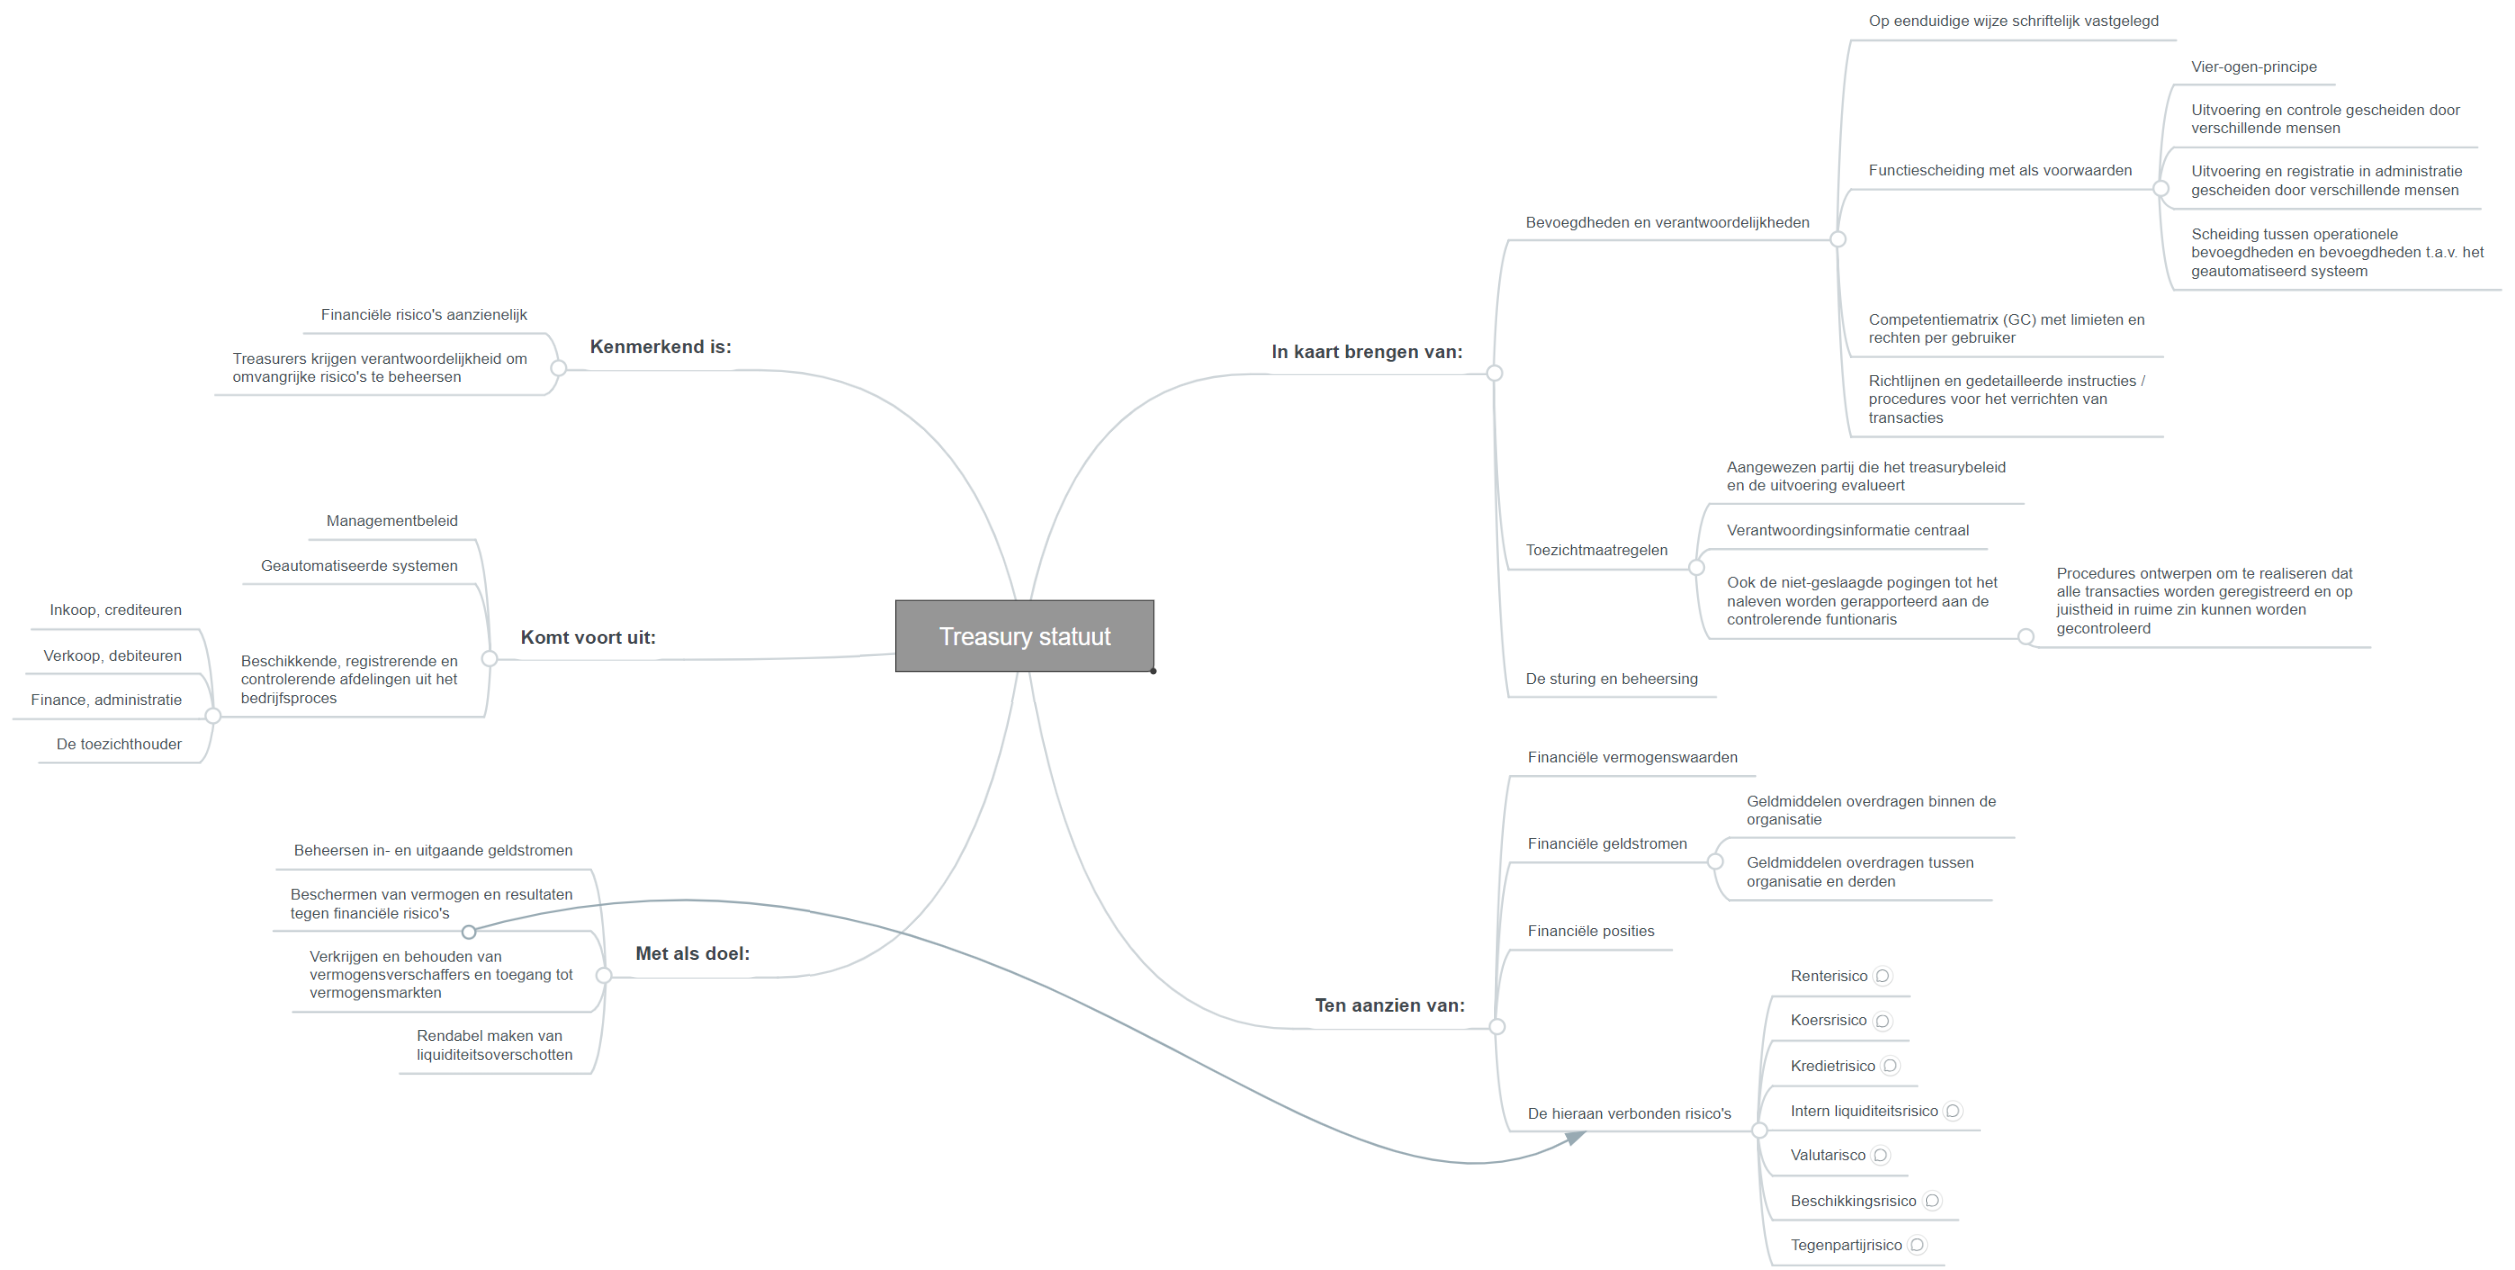
\includegraphics[angle=90,width=0.795\textwidth]{treasury}
    \label{fig:mmtreasury}
\end{figure}

\newpage
\stepcounter{bijlage}
\subsection*{\hypertarget{bij:inkoopproces}{Bijlage \thebijlage}: het inkoopproces (voorwaardelijk)}
\addcontentsline{toc}{section}{Bijlage \thebijlage: het inkoopproces (voorwaardelijk)}
\begin{figure}[!ht]
    \centering
    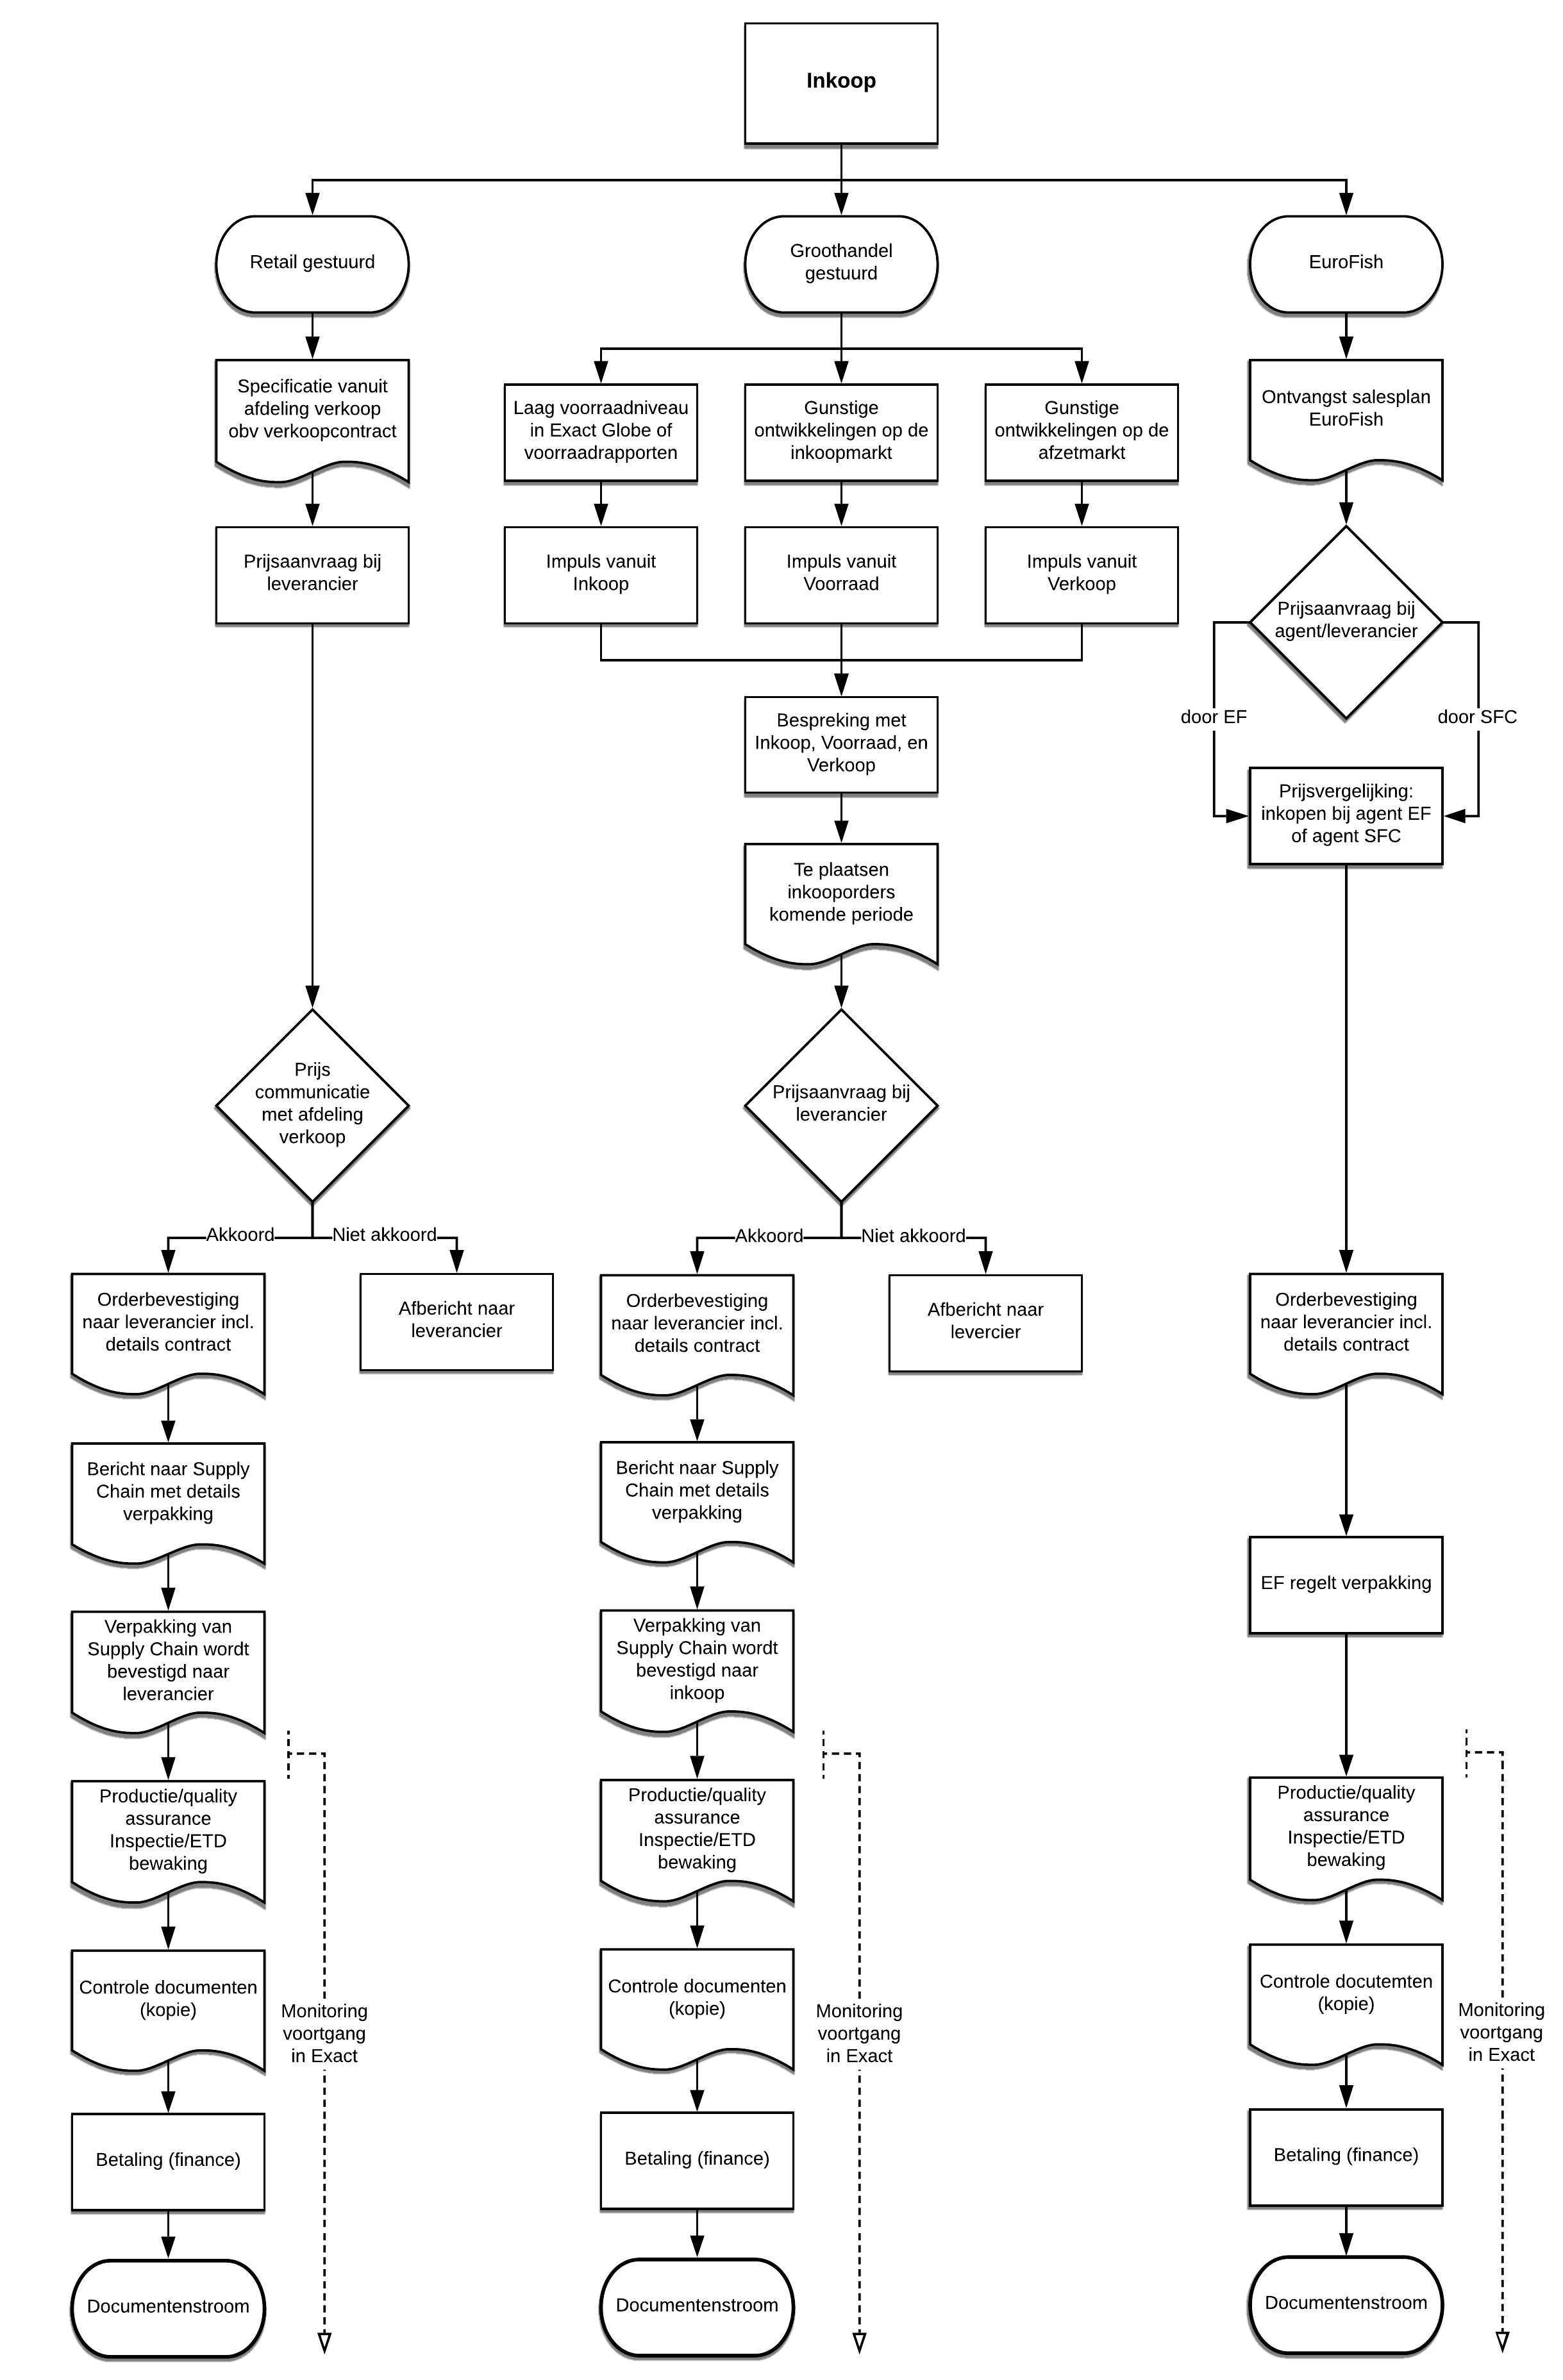
\includegraphics[width=1\textwidth]{inkoopproces}
    \label{fig:inkoopproces}
\end{figure}
